The web server runs on port 8080, which means to access it, you'll need to
navigate to \texttt{http://[YOUR\_HESTIA\_IP]:8080/}  When there, there will
be two options for which user interface (UI) to use: Basic UI or Paper UI.
The Basic UI is documented in section \ref{Basic UI} while the Paper UI is
covered by section \ref{Paper UI}.  This choice can be seen in figure
\ref{fig:ui-choice}.

\begin{figure}
\centering
\begin{subfigure}{0.32\textwidth}
  \centering
  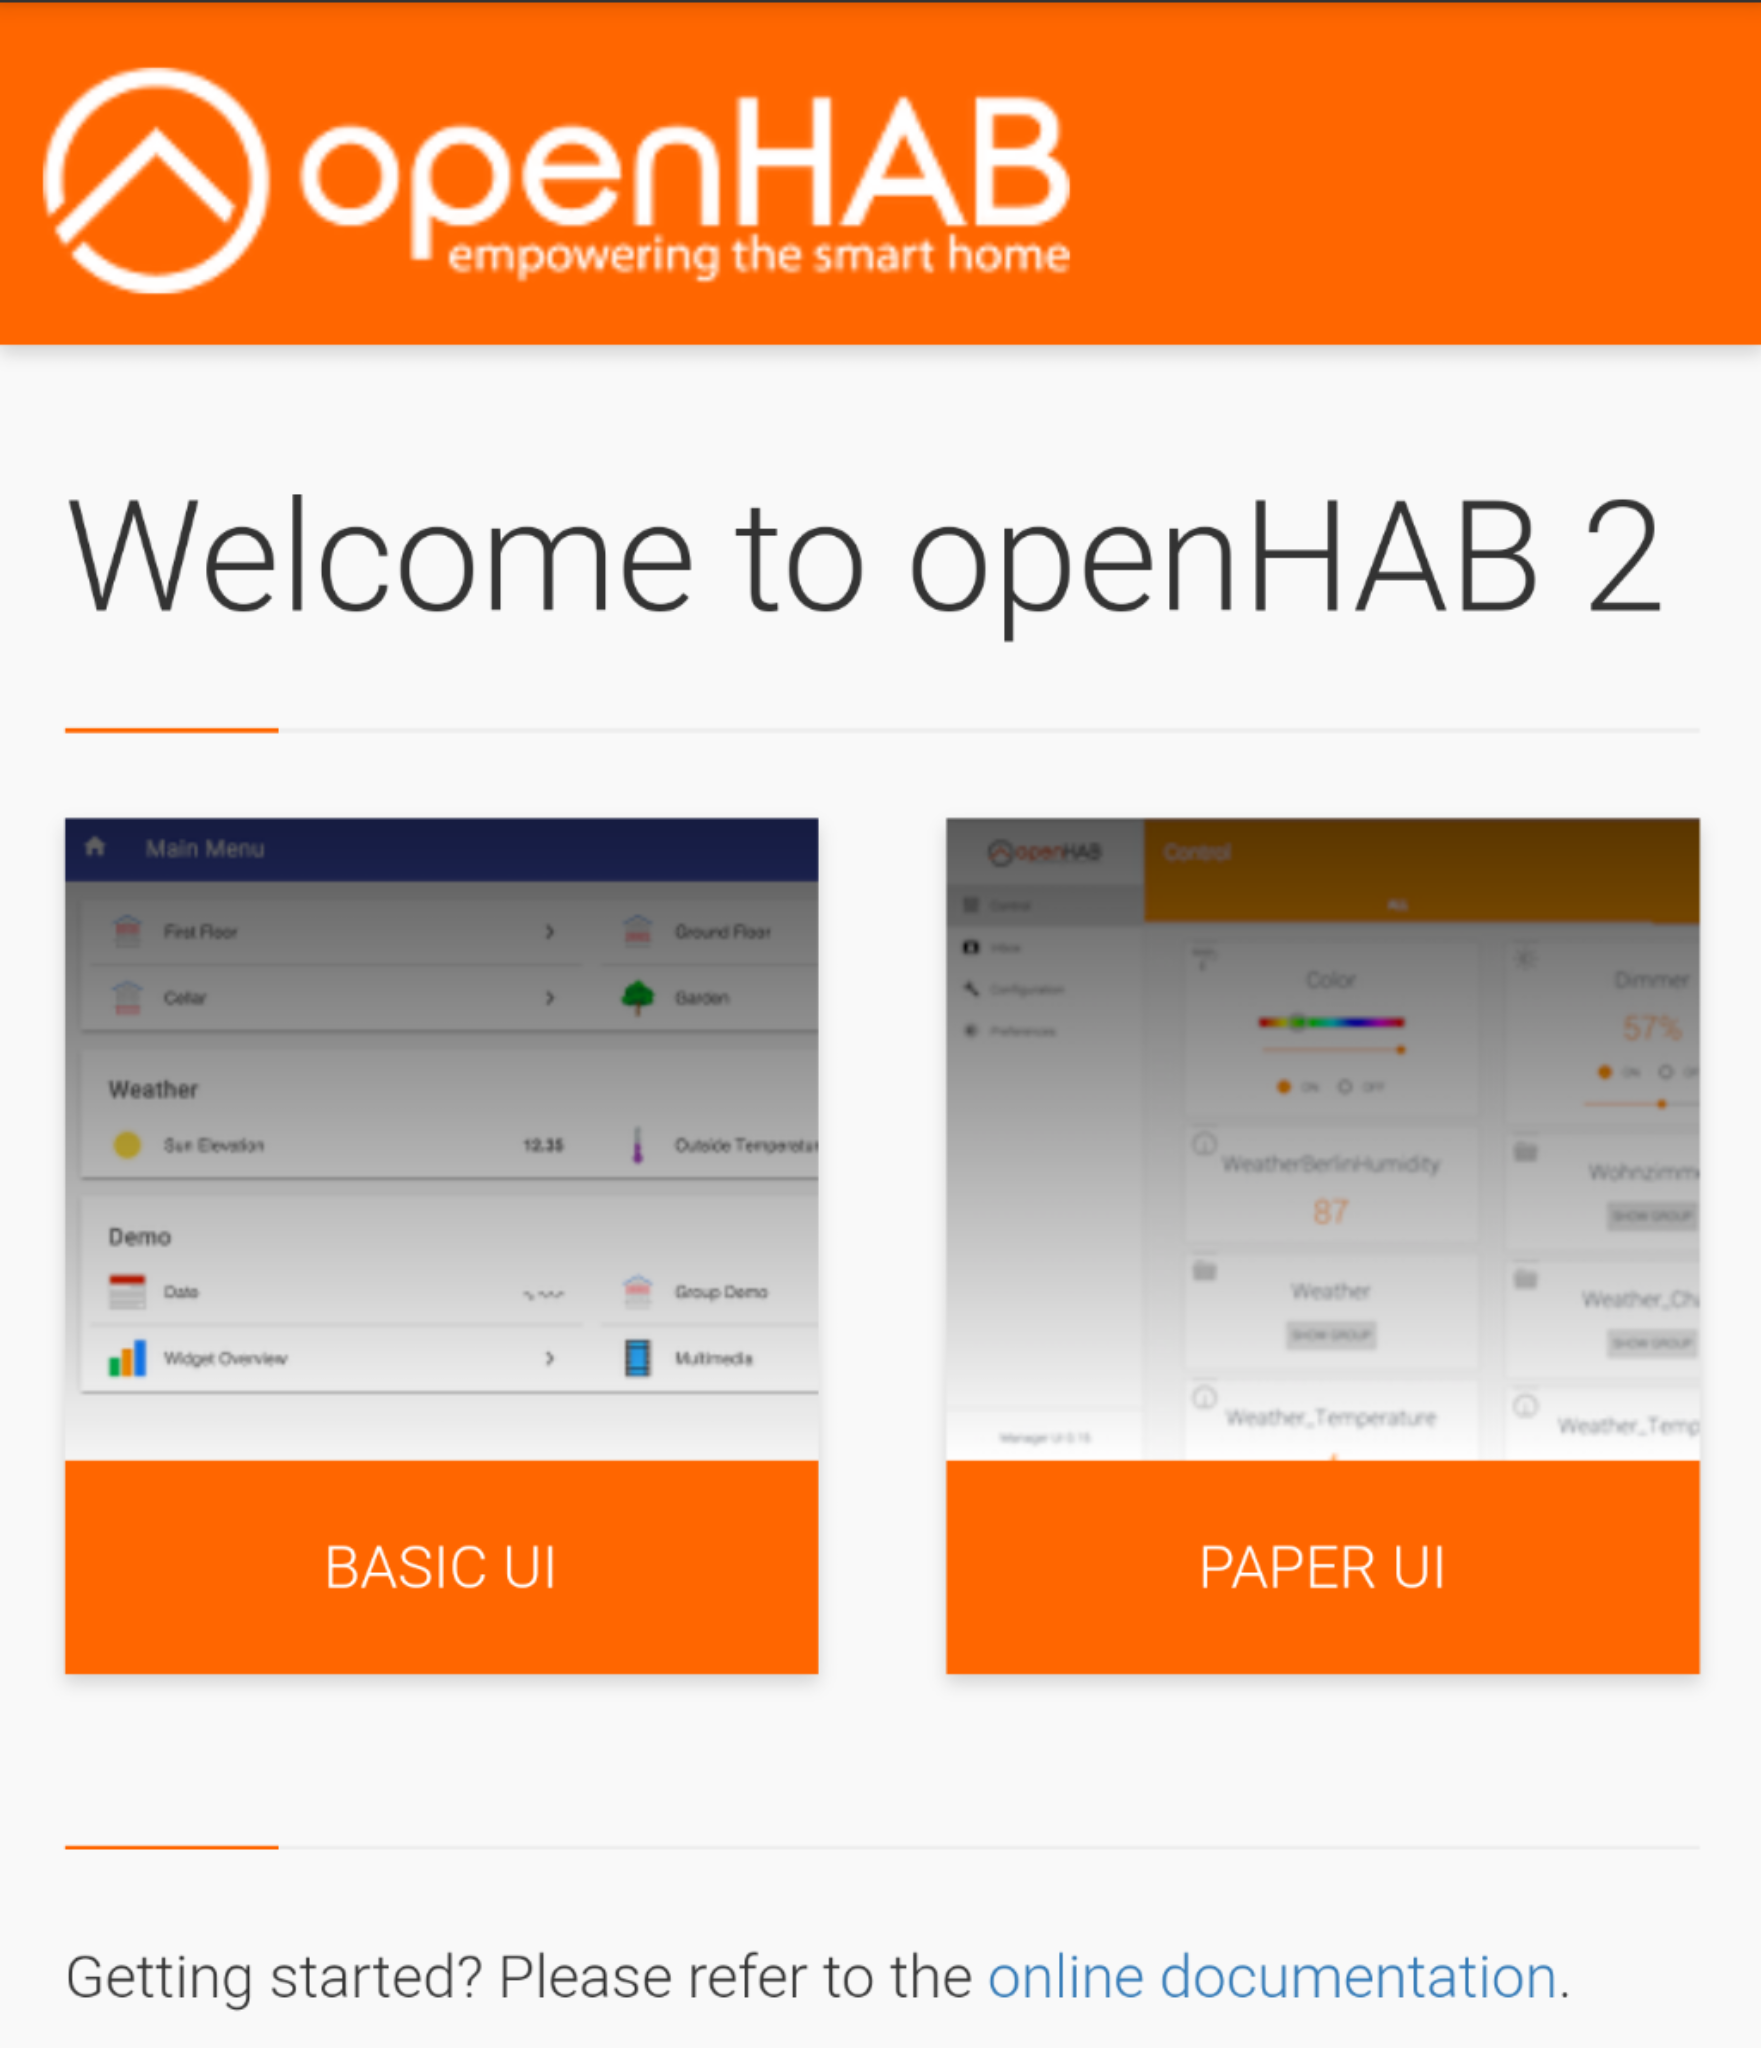
\includegraphics[width=.75\linewidth]{img/ui-choice.png}
  \caption{User Interface Choices}
  \label{fig:ui-choice}
\end{subfigure}%
\begin{subfigure}{0.33\textwidth}
  \centering
  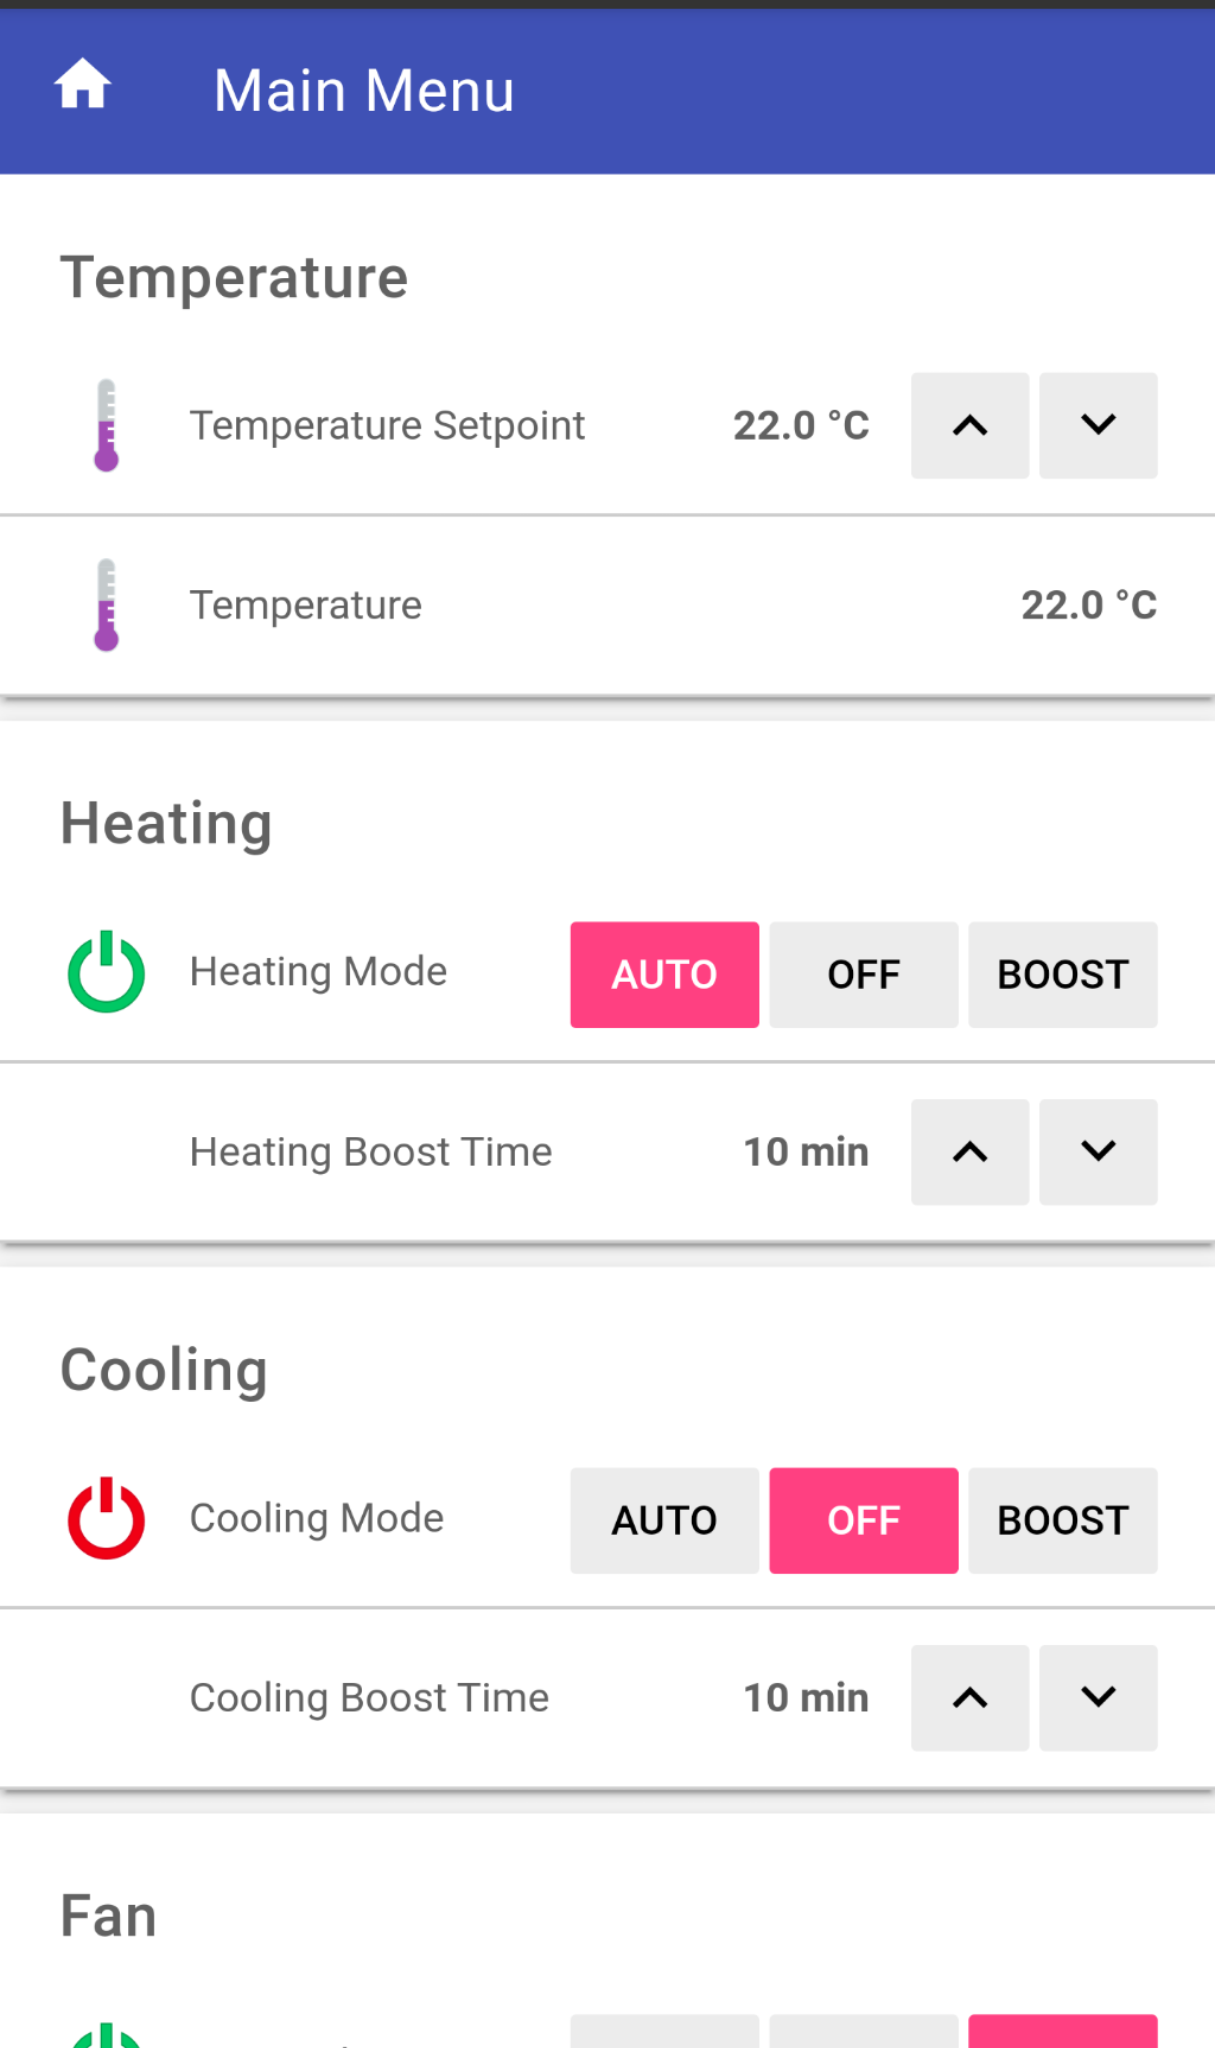
\includegraphics[width=.75\linewidth]{img/ui-main-menu1.png}
  \caption{Main Menu}
  \label{fig:ui-main-menu1}
\end{subfigure}
\begin{subfigure}{0.33\textwidth}
  \centering
  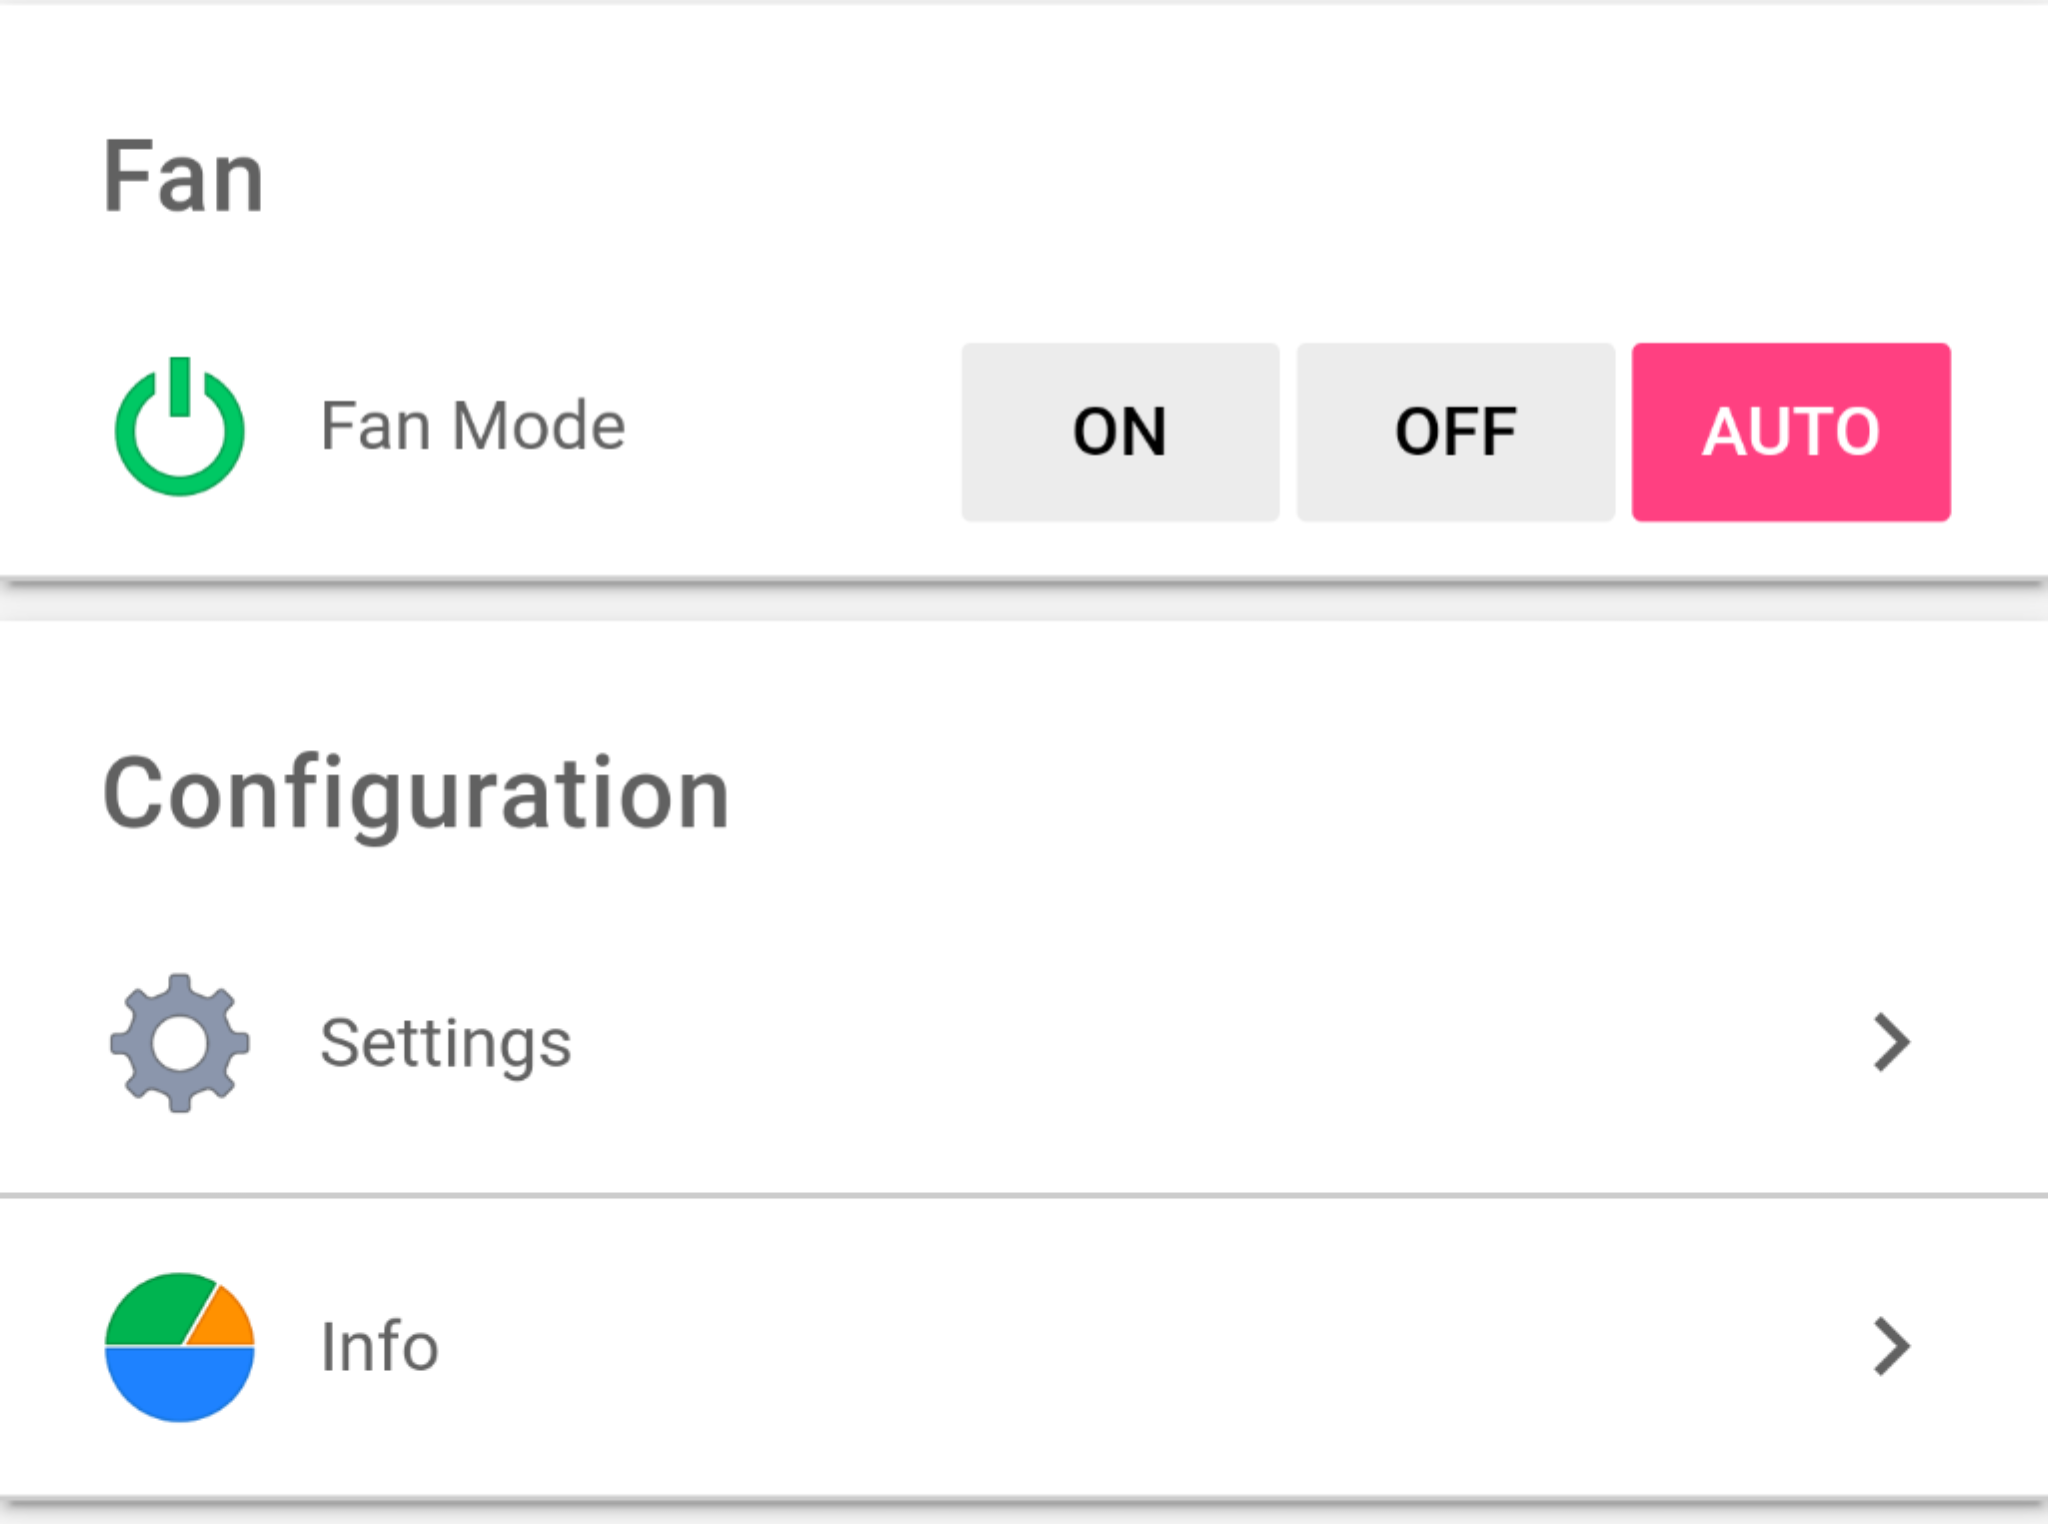
\includegraphics[width=.75\linewidth]{img/ui-main-menu2.png}
  \caption{Bottom of Main Menu}
  \label{fig:ui-main-menu2}
\end{subfigure}%

\begin{subfigure}{0.32\textwidth}
  \centering
  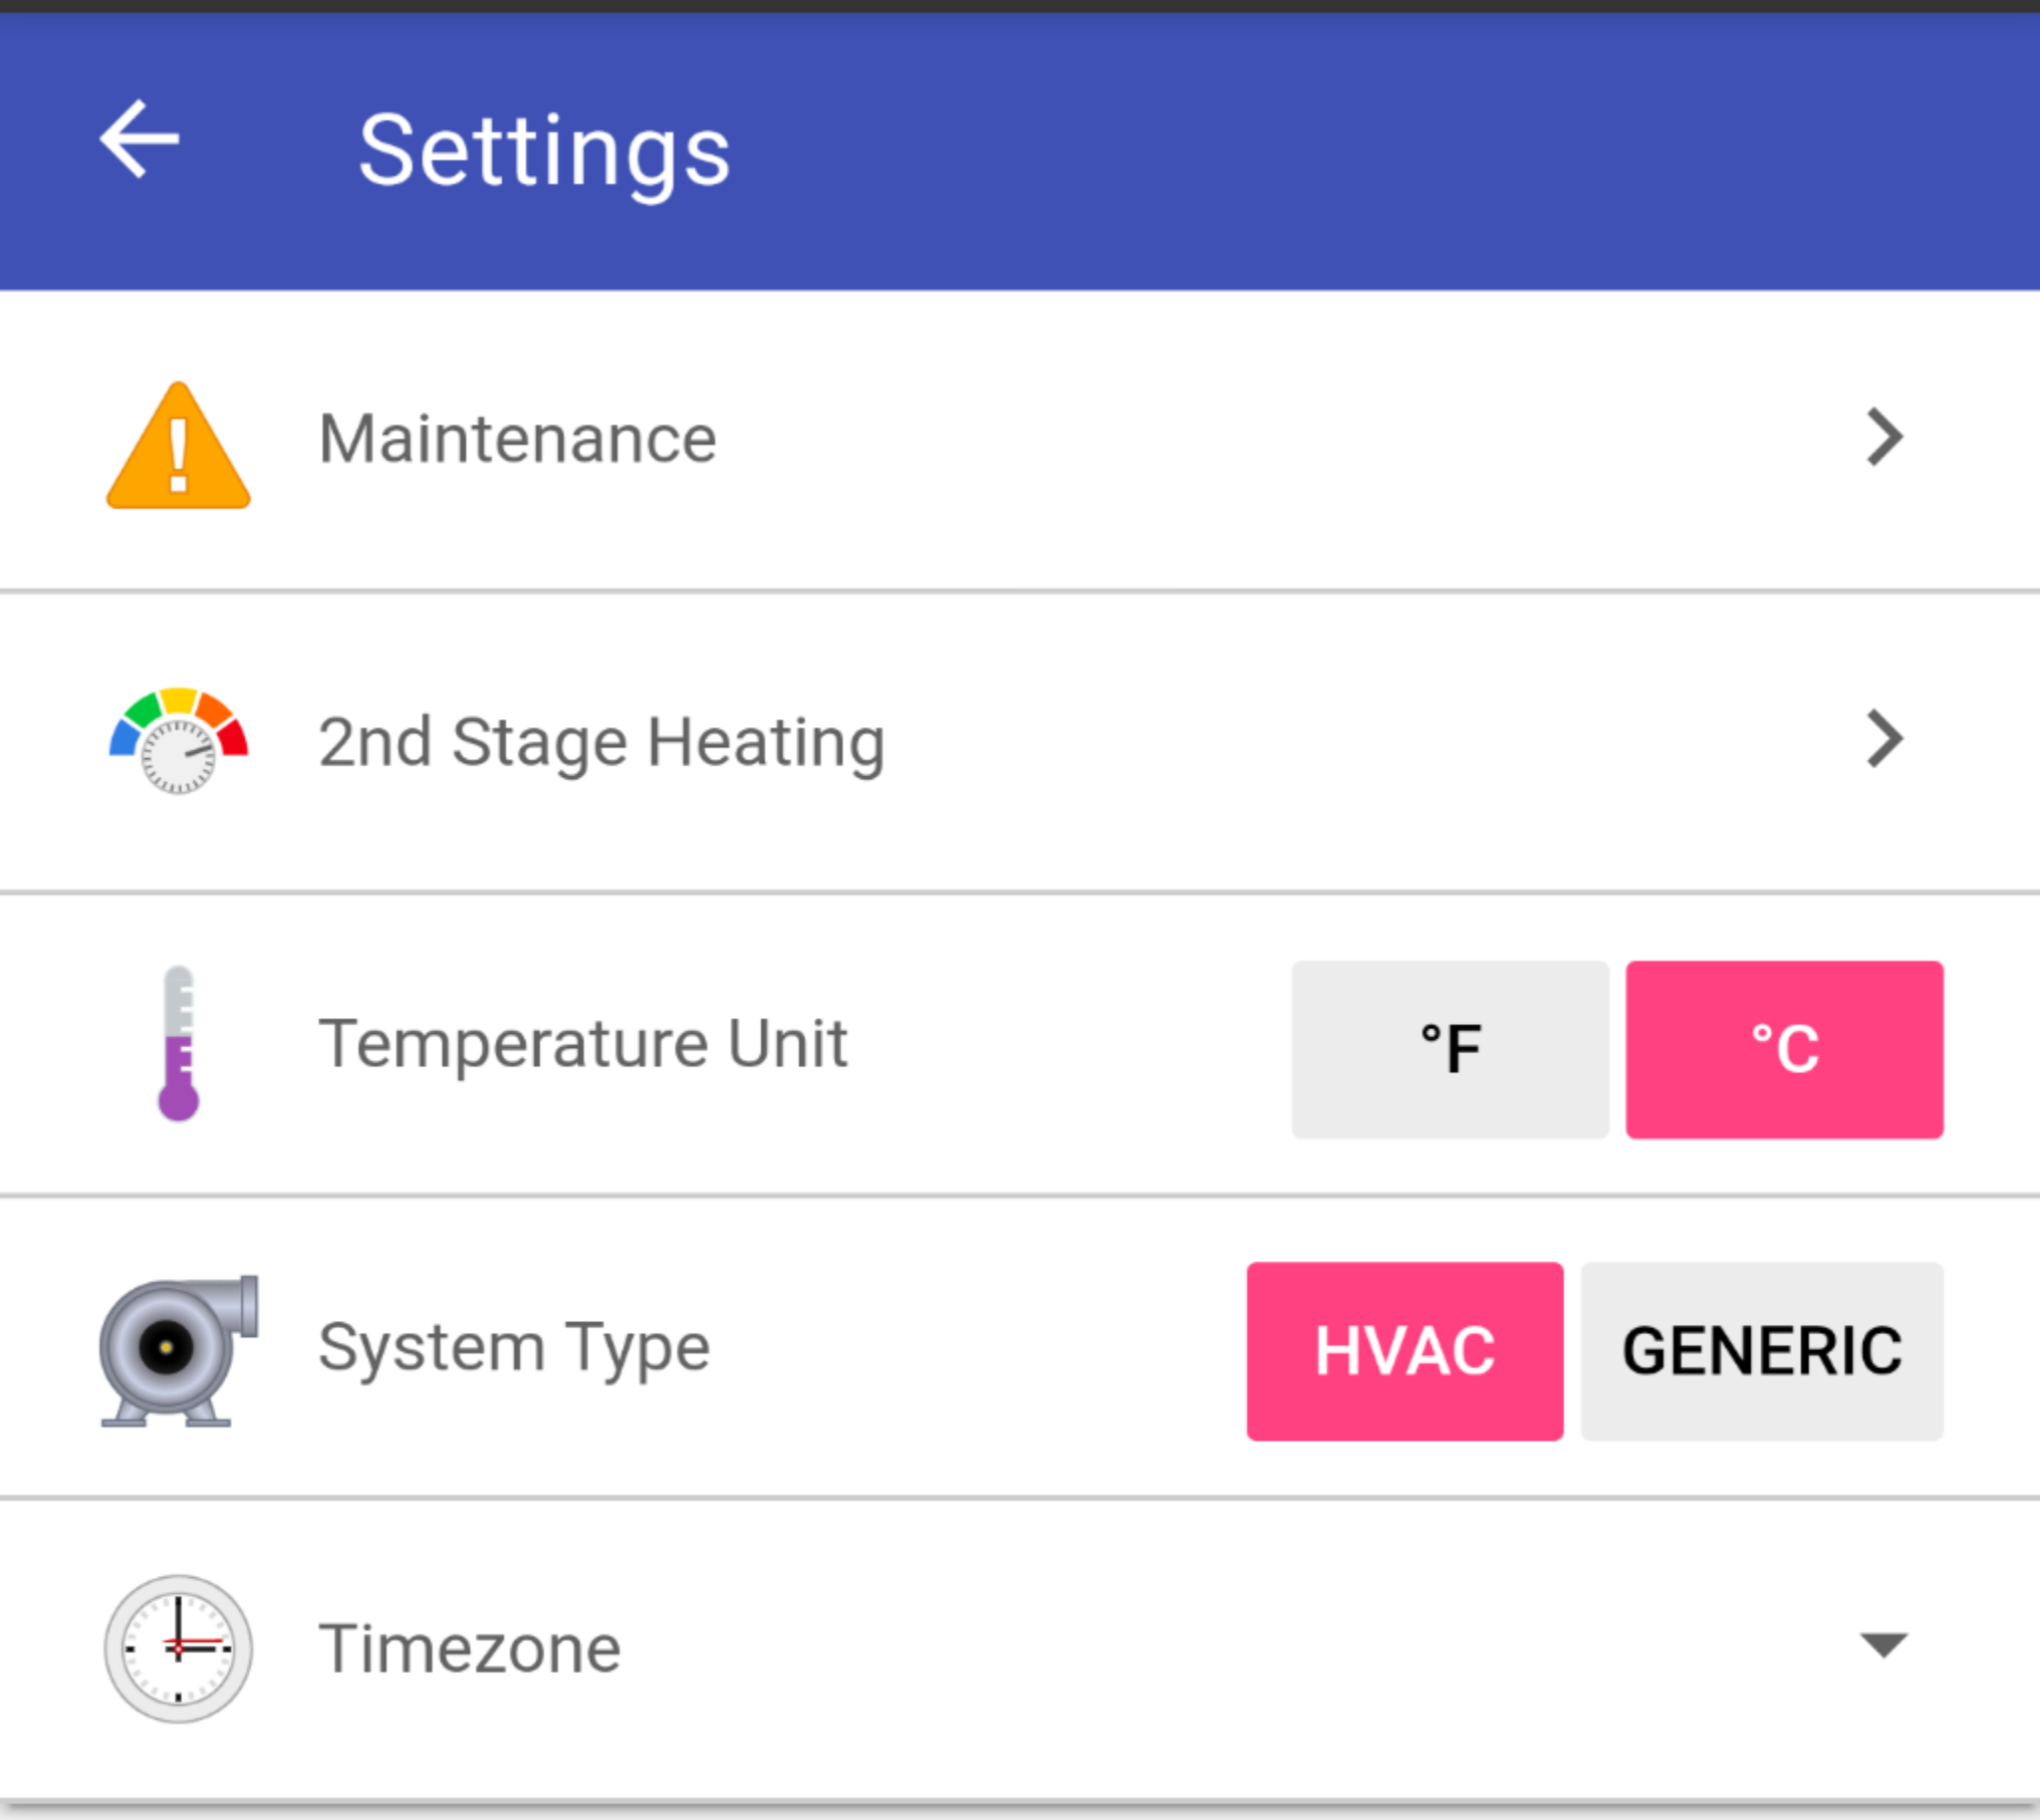
\includegraphics[width=.75\linewidth]{img/ui-settings.png}
  \caption{Settings}
  \label{fig:ui-settings}
\end{subfigure}
\begin{subfigure}{0.33\textwidth}
  \centering
  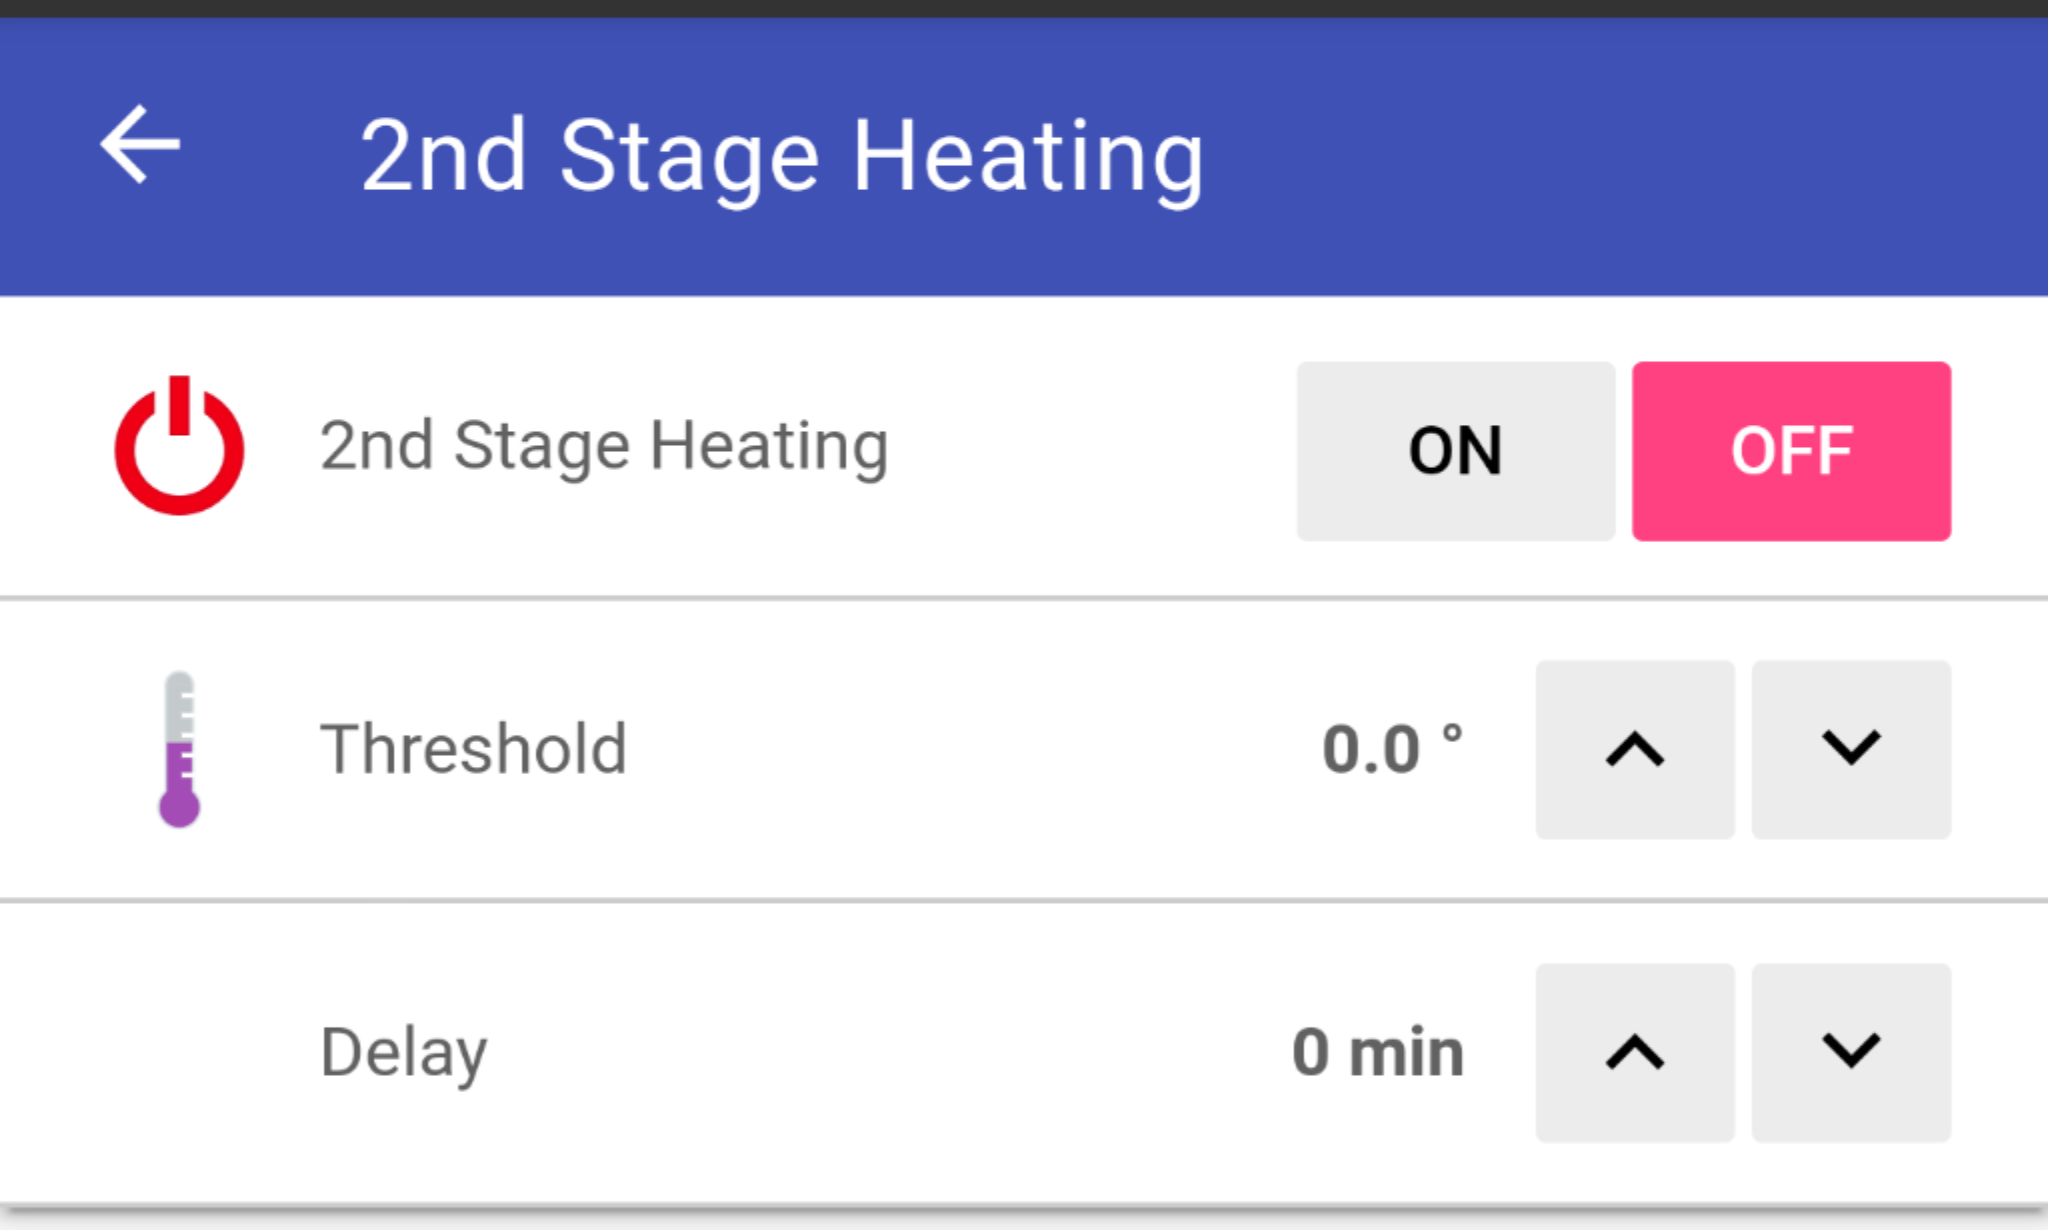
\includegraphics[width=.75\linewidth]{img/ui-2nd-stage-heating.png}
  \caption{2nd Stage Heating}
  \label{fig:ui-2nd-stage-heating}
\end{subfigure}%
\begin{subfigure}{0.33\textwidth}
  \centering
  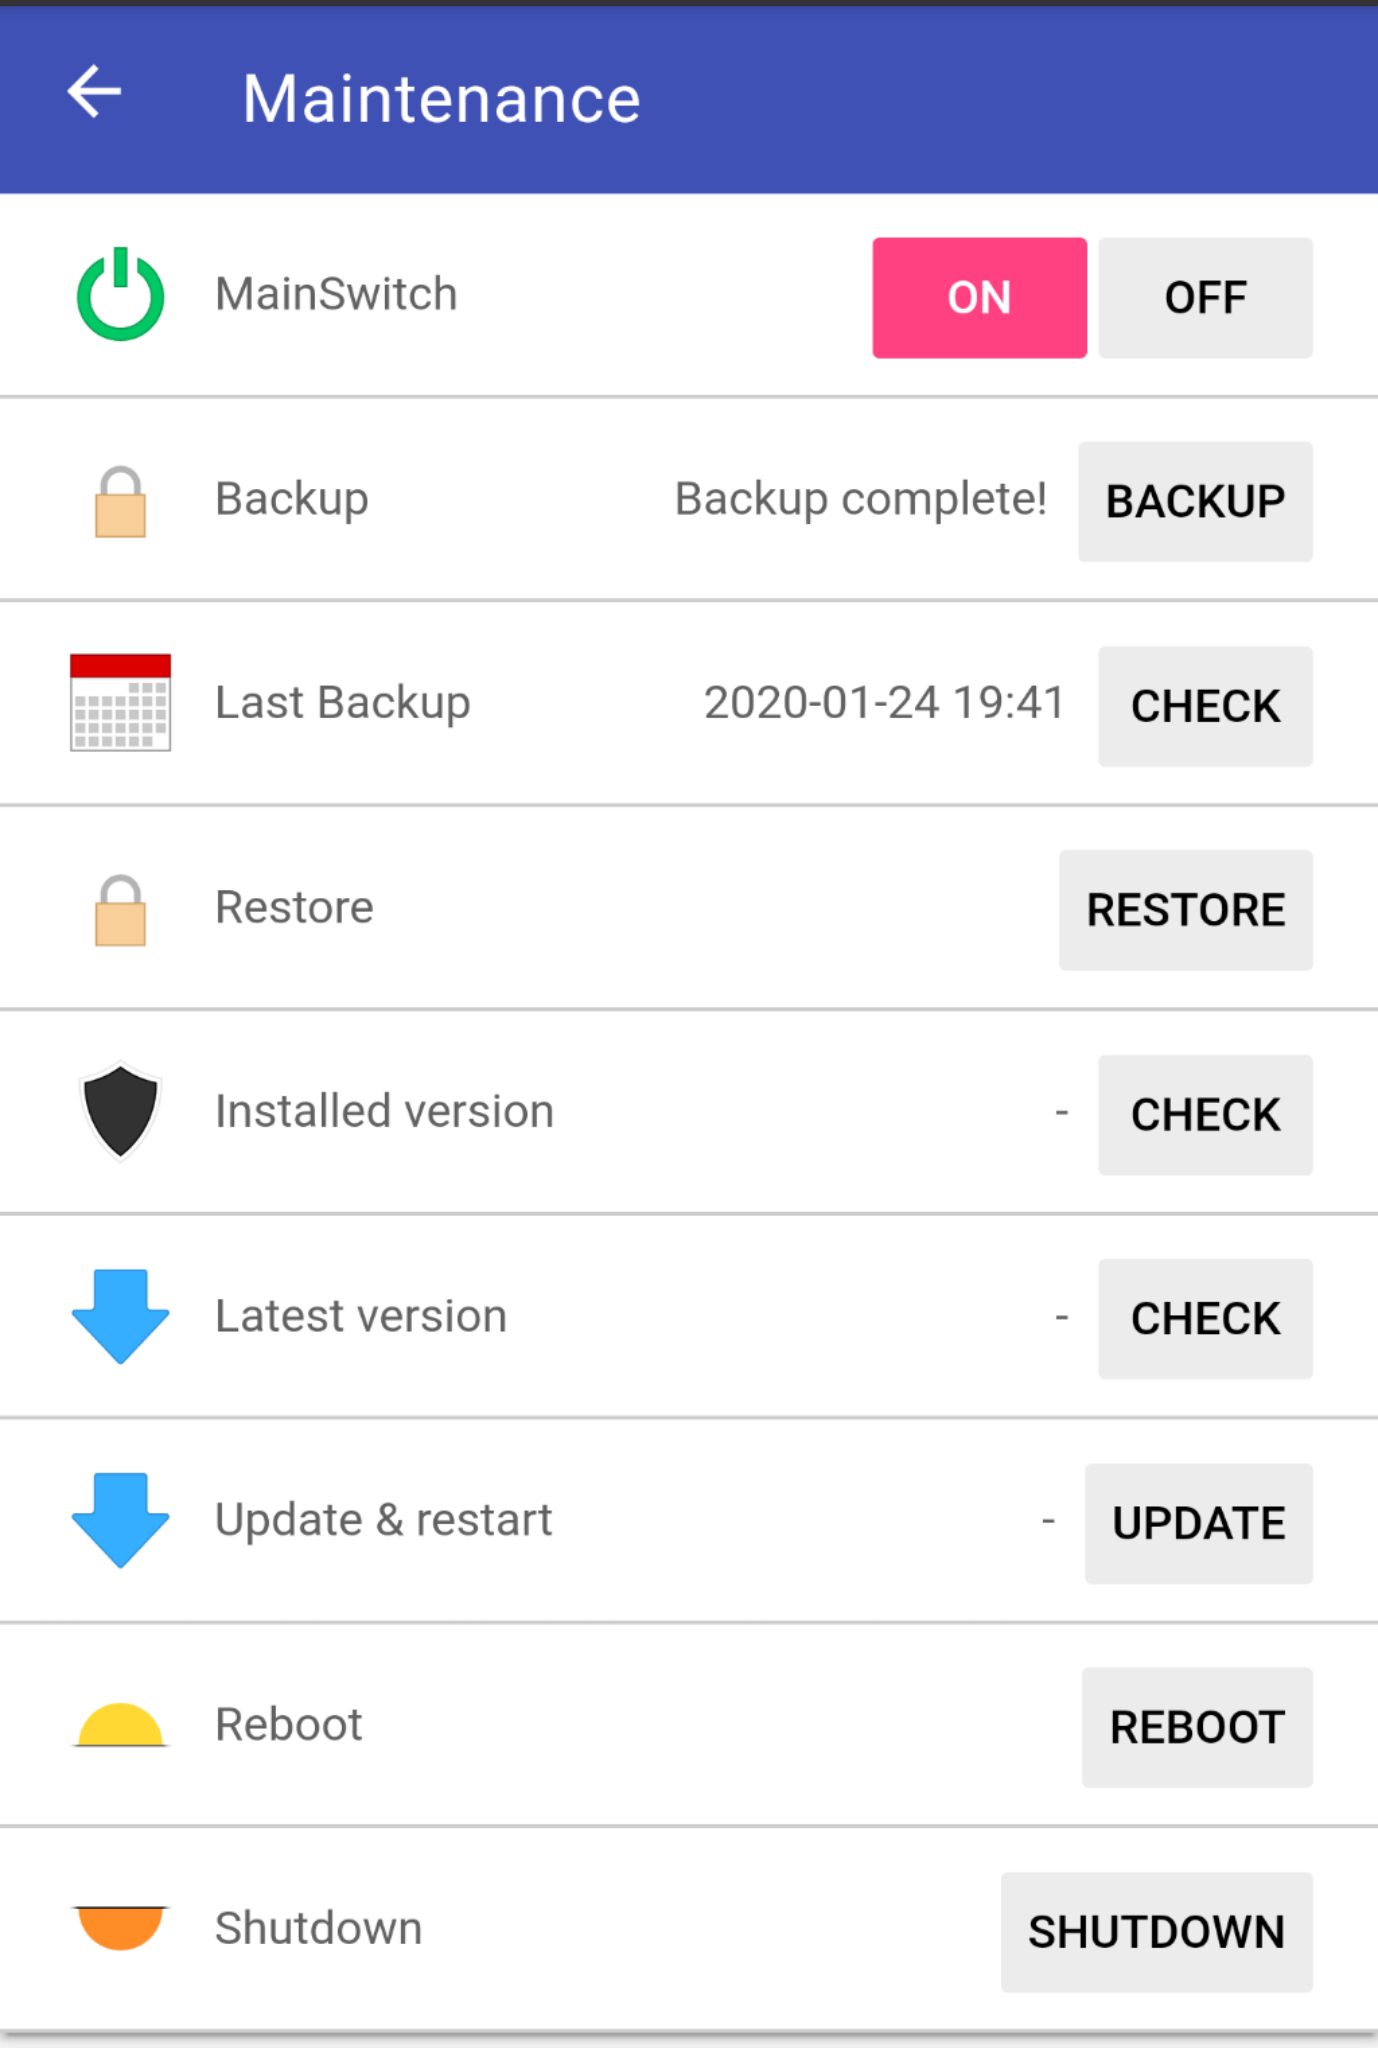
\includegraphics[width=.75\linewidth]{img/ui-maintenance2.png}
  \caption{Maintenance Menu After a Backup}
  \label{fig:ui-maintenance2}
\end{subfigure}
\caption{fig:Web UI}
\label{fig:Web UI}
\end{figure}


\subsubsection{Basic UI} \label{Basic UI}
The basic UI is for controlling the thermostat from your device (phone, laptop,
tablet, desktop, etc.).  This UI covers the same functionality as the
touchscreen (see section \ref{Touchscreen} for more details), plus the ability
to do maintainence tasks such as taking backups, updating the software, and
shutting down the HestiaPi in case you need to do hardware maintainence.

Figures \ref{fig:ui-main-menu1} and \ref{fig:ui-main-menu2} show the main menu.
The heating and cooling can be adjusted similar to the way as is done using the
touch screen on the HestiaPi.  In the settings menu (figure
\ref{fig:ui-settings}), there are some additional features which are not
accessible via the touchscreen interface.  This includes switching from Celsius
to Fahrenheit, settings your time zone and if your system has second stage
heating it can be configured here (as seen in figure
\ref{fig:ui-2nd-stage-heating}).

The maintenance menu allows for backups, updates, and shutting down the pi,
which is typically only necessary when taking off the LCD screen to do physical
maintenaince or upgrades.  When the backup button is pressed, it will update
both the backup field to show that it is done as well as the latest backup
field with the date and time of the latest backup, as shown in figure
\ref{fig:ui-maintenance2}.

\subsubsection{Paper UI} \label{Paper UI}
The paper UI is used for advanced configuration settings.  This section will be
expanded in the future, but in the meantime, you can read the
\href{https://www.openhab.org/docs/}{OpenHAB documentation}.
